\subsection{Smoothing}\label{sec:smoothing}

Smoothing an image means reducing the impact of transitions.
The process of smoothing involves applying a kernel to an image using convolution.
Smoothing is applied to an image in order to reduce the noise in the image such that only the important features are left in the data.
A wide range of kernels can be used for smoothing, but in this report only the Gaussian kernel is considered.
Furthermore, the kernels considered here all have a sum of one, such that the brightness of the image is unchanged.

When applying a smoothing filer, the neighbouring pixels to the smoothed are added a contribution from the smoothed.
The process of smoothing hence widens the digits, as seen in figure \ref{fig:effect_smooth}, and this should give a better chance of two characters overlapping.
The danger is that too much smoothing blurs the whole image and hence remove the features in the data that is used to compare and identify the characters.

\begin{figure}[H]
\centering
	\begin{subfigure}[b]{0.2\textwidth}
	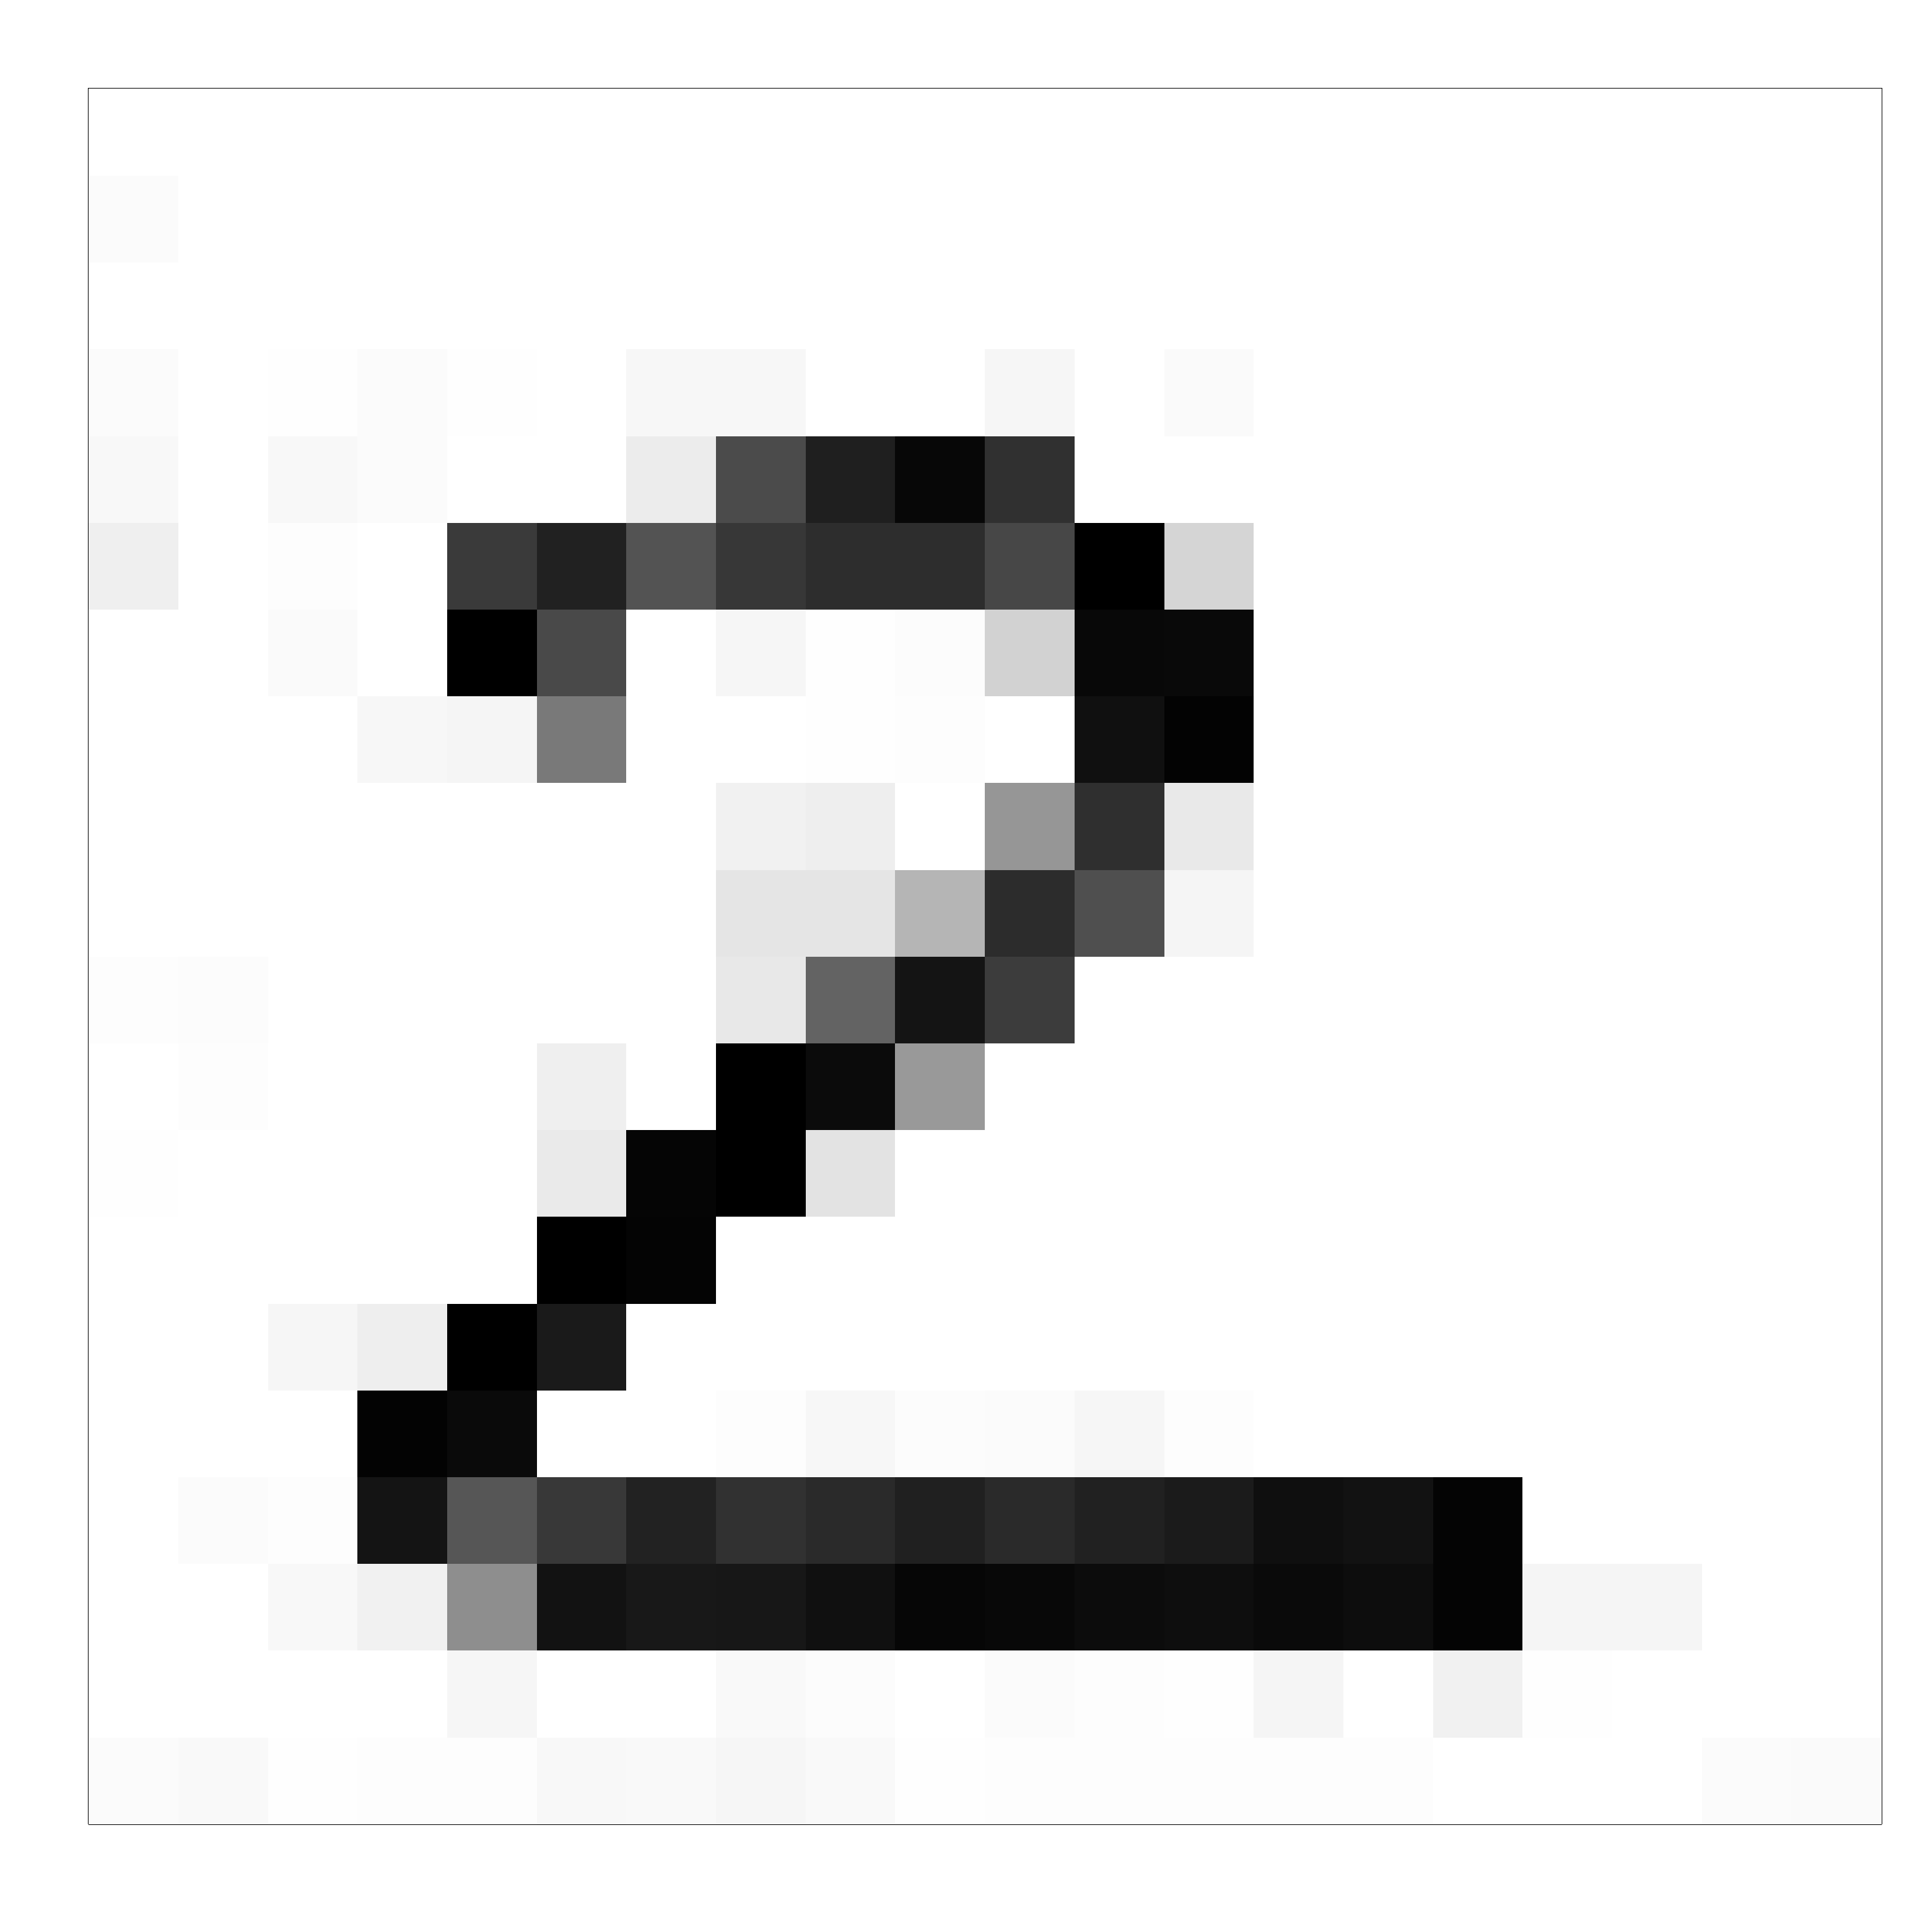
\includegraphics[width=\textwidth]{graphics/smooth_none}
	\caption{Raw image.}
	\end{subfigure}
	\qquad
	\begin{subfigure}[b]{0.2\textwidth}
         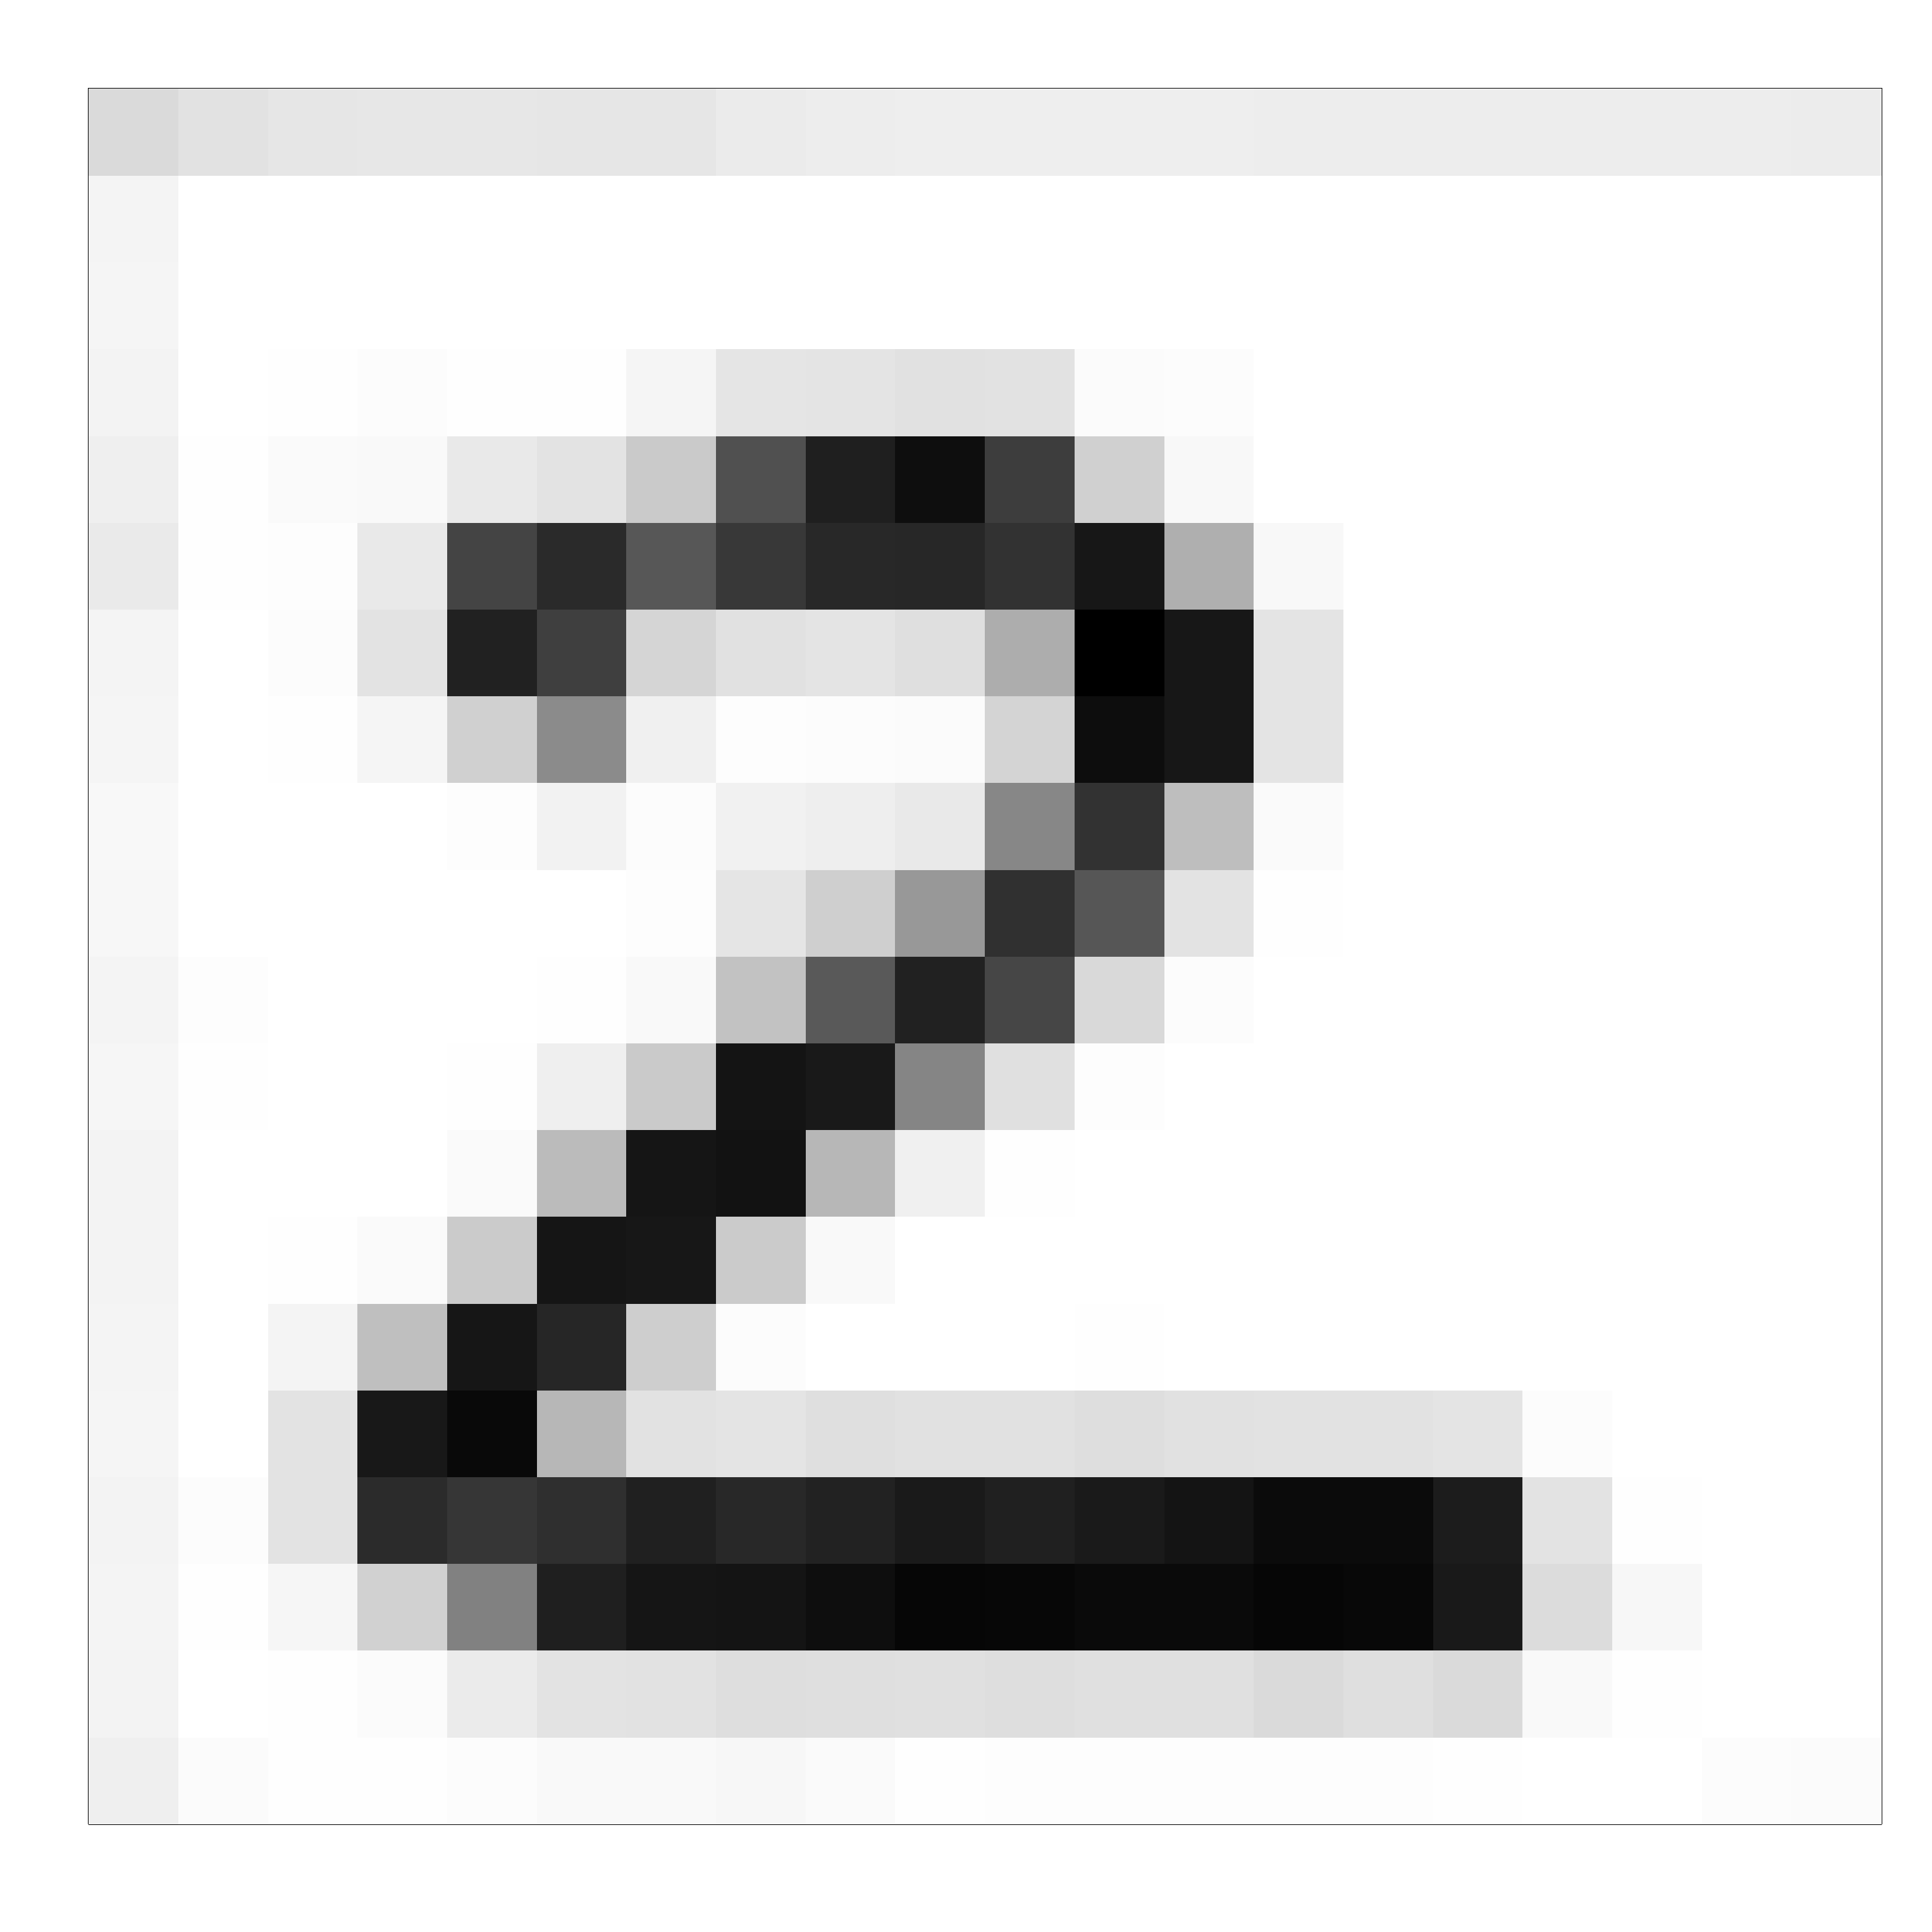
\includegraphics[width=\textwidth]{graphics/smooth_05_5}
         \caption{\(\sigma = 0.5\).}
	\end{subfigure}
	\qquad
	\begin{subfigure}[b]{0.2\textwidth}
         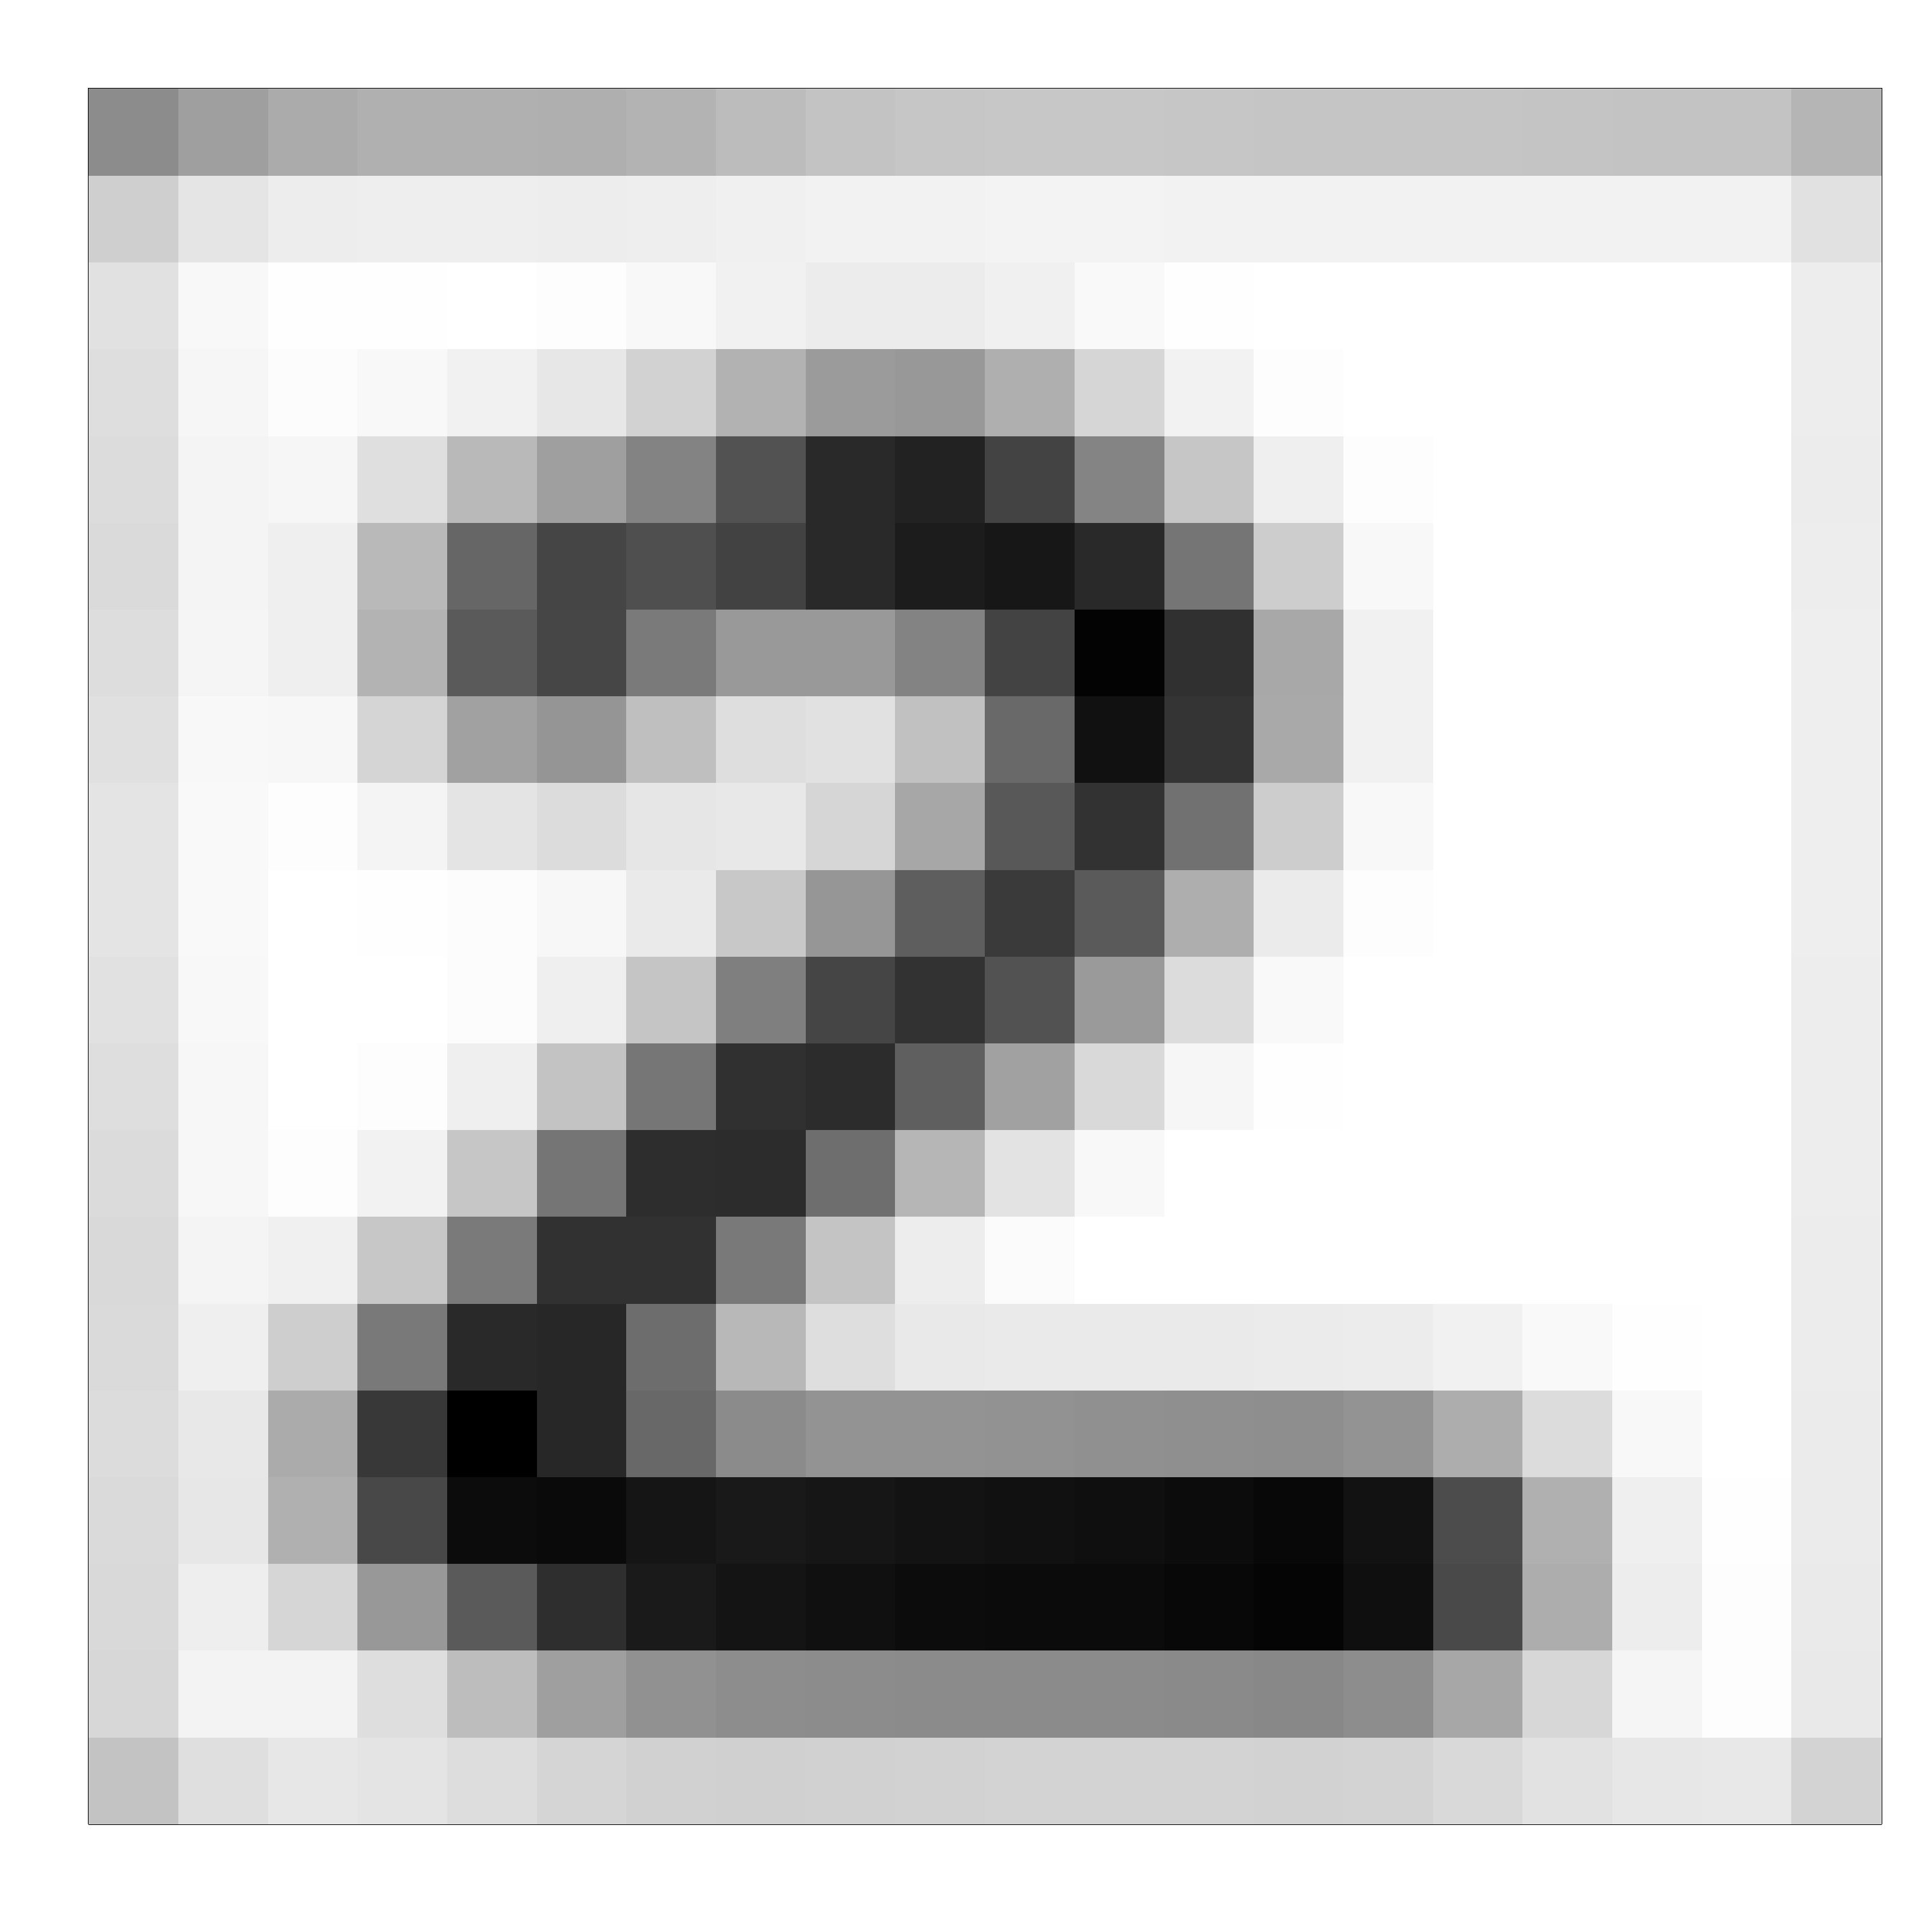
\includegraphics[width=\textwidth]{graphics/smooth_1_5}
         \caption{\(\sigma = 1\).}
	\end{subfigure}
	\qquad
	\begin{subfigure}[b]{0.2\textwidth}
         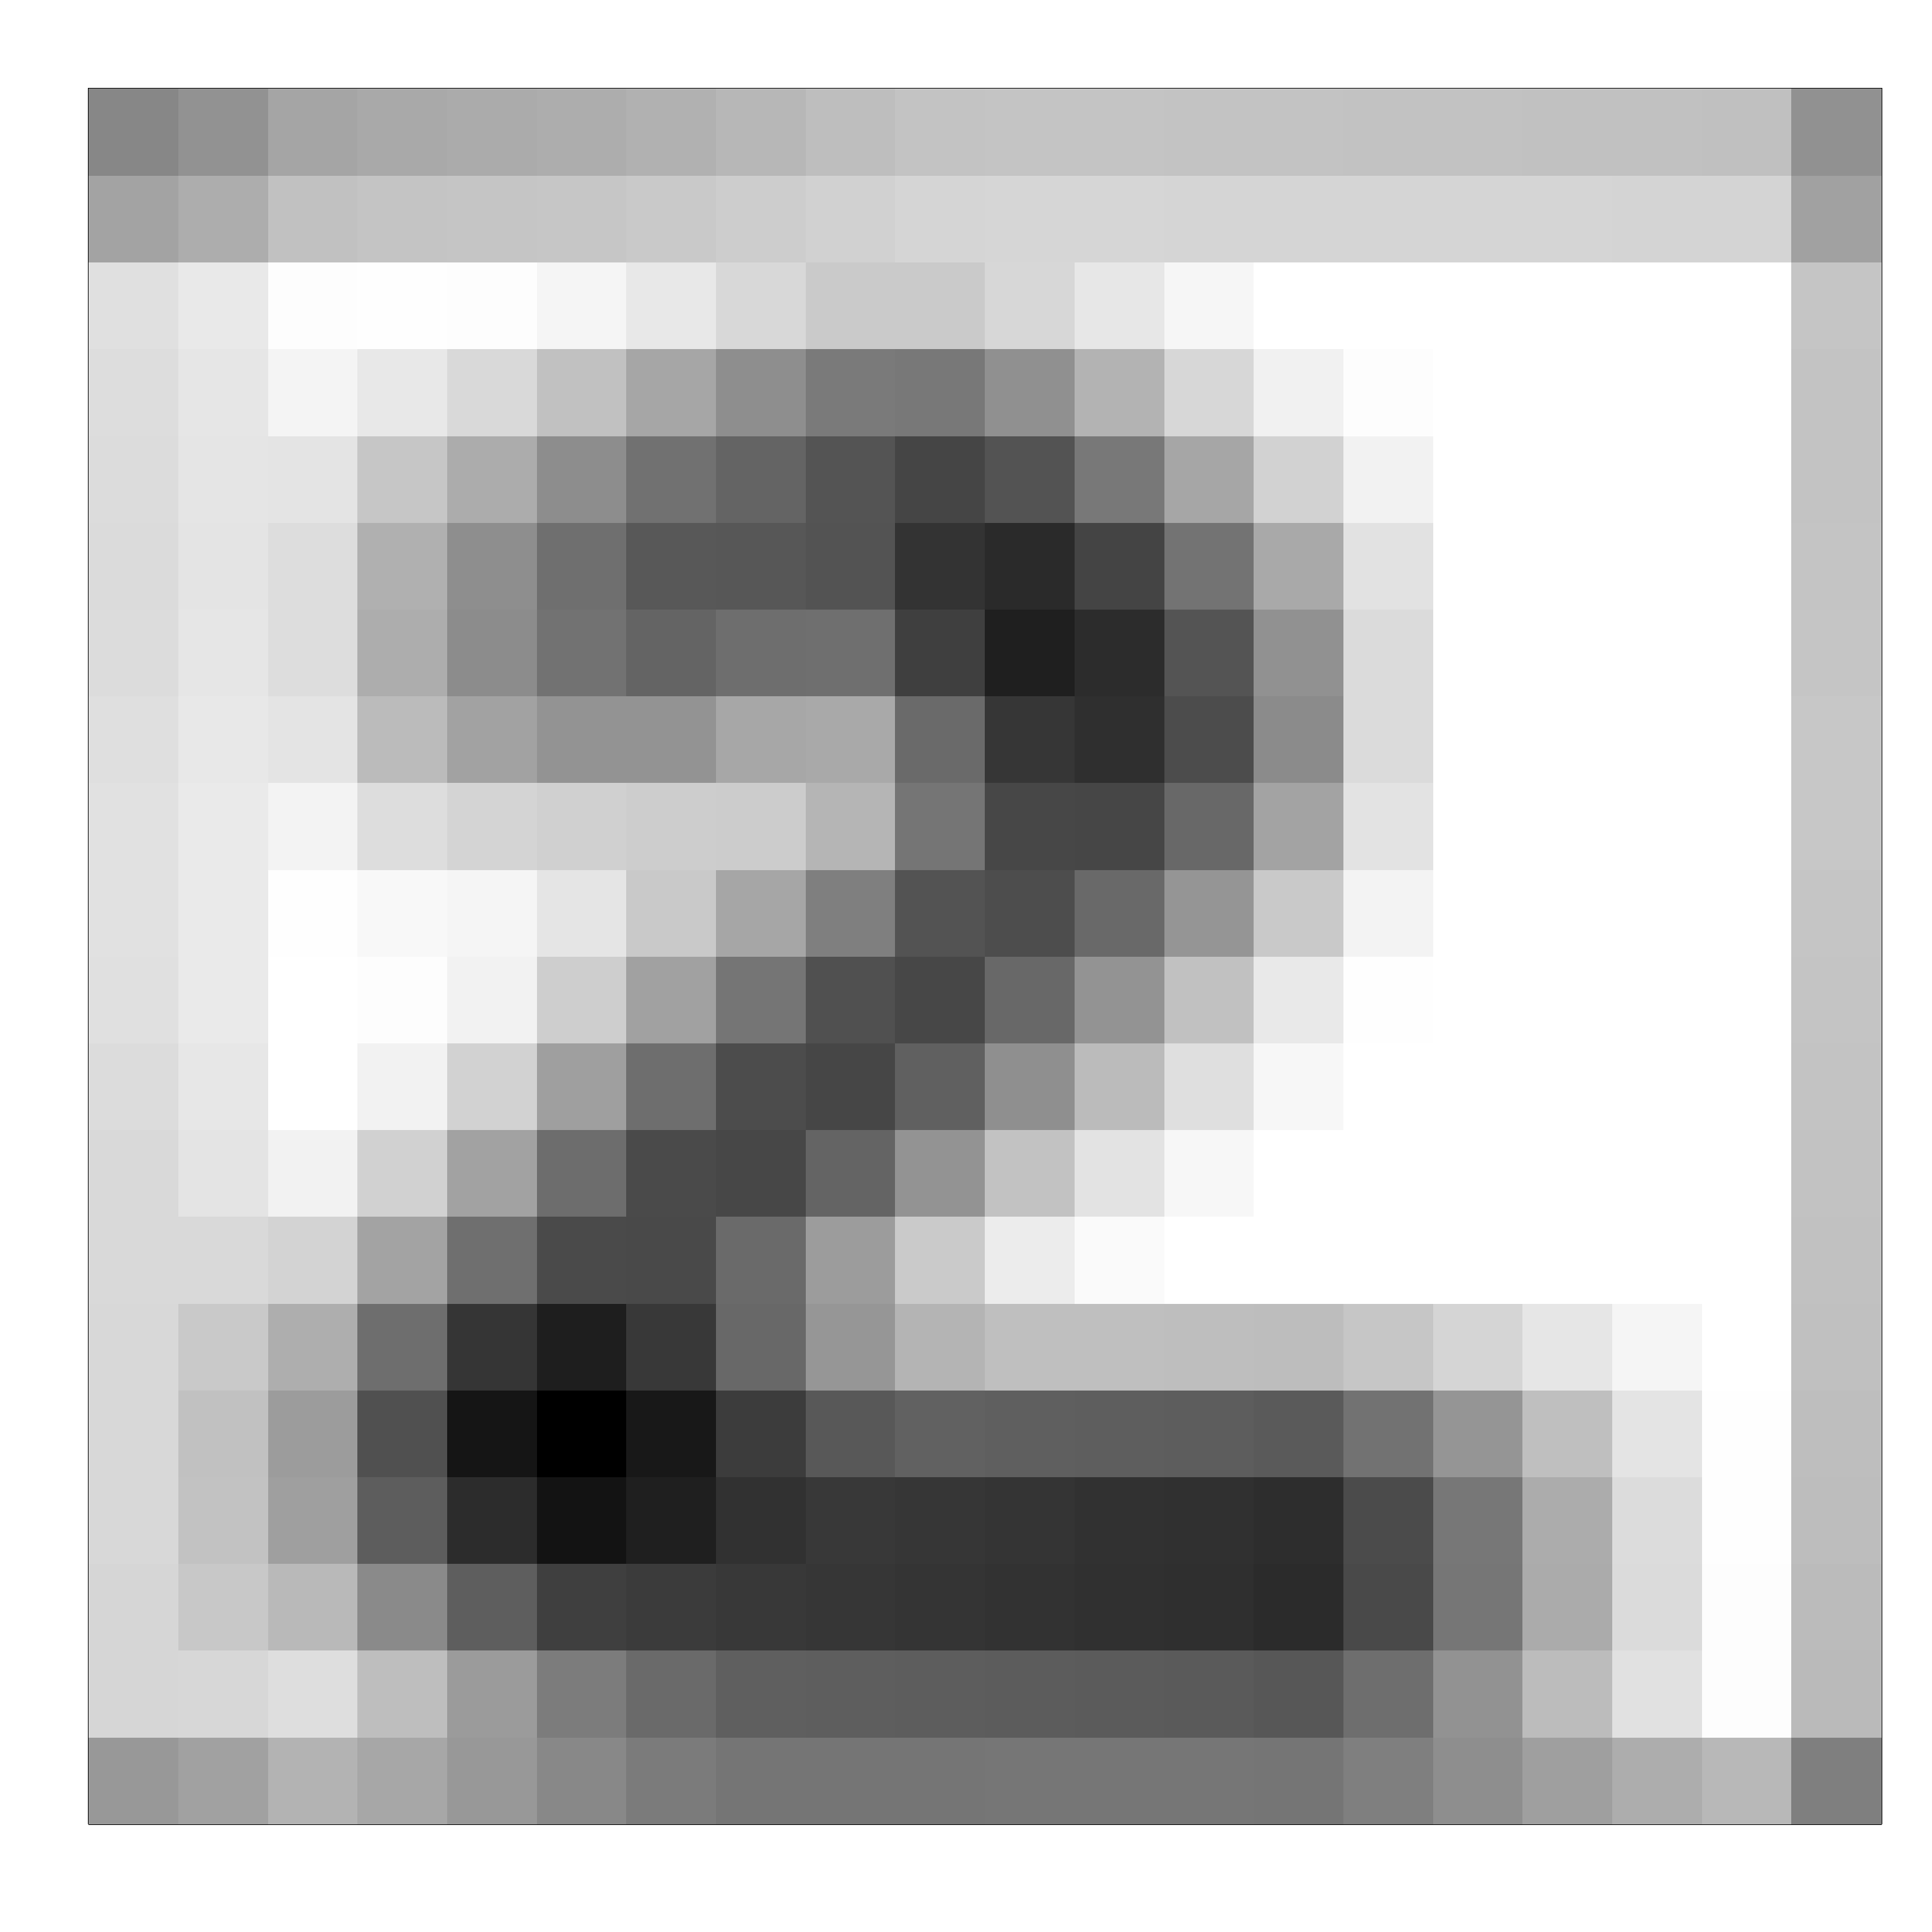
\includegraphics[width=\textwidth]{graphics/smooth_2_5}
         \caption{\(\sigma = 2\).}
	\end{subfigure}
\caption[Effects of smoothing on image.]{Illustration of Gaussian smoothing. All kernels are 5x5.}
\label{fig:effect_smooth}
\end{figure}

A Gaussian distribution (also referred to as a normal distribution) is a naturally occurring distribution which is found when a random result occurs around a mean. 
The $\sigma$ signifies the deviation of the distribution. 
The 2D equation of a Gaussian distribution is shown in equation \ref{eq:gauss}. 

\begin{equation}
G(x,y) = \frac{1}{2\pi \sigma^2} e^{- \frac{x^2+y^2}{2\sigma^2}} \label{eq:gauss}
\end{equation}

Using the Gaussian filter to smooth an image will weigh the distance to the pixel.
A small $\sigma$ will make a small deviation and thus heavily weigh the center pixel.
The Gaussian filter is the one applied in figure \ref{fig:effect_smooth}.

%Applying a smoothing function can give the image an advantage when using the nearest neighbour analysis.

%The results of the filtering methods were also compared to the raw image with 100, 200 and 300 DPI.
%These results are compared with an averaging filter (avg) which takes the average of the four neighbouring pixels and a Gaussian filter (G) with different values for sigma.
%These tests were done 10 times, using cross validation, and the mean of each success rate is plotted in figure \ref{fig:smooth}. 
%Since the variance is too small to be seen in the figure the mean and variance is shown in table \ref{tb:smooth}.
%The averaging filter does not give a measurable different result from not using a filter.
%The Gaussian filter does improves the success rate for some values of sigma, but a larger $\sigma$ makes it worse.

